%Foundations chapter
% contains fundamental and basic theories to approach the content later
%		(LinAlg)Notation (math framework for QM)
%		QM
%			Introduce first abstract QM on Hilbert space and then dirac
%		Information theory


\section{Mathematical Framework (for QM)}
	%TODO Correct and reformulate
	
		In order to understand subsequent sections of this thesis a basic knowledge of the mathematical framework behind quantum mechanics is needed.
		 It is also important to specify a standard notation as used in literature.
	
%	\begin{enumerate}
%	\item Dirac's braket notation
%	\item Inner/(Outer) product
%	\item Linear operator
%	\item Adjoints and Hermitian operators
%	\item Pauli matrices
%	\item Tensor Product and tensor space
%	\end{enumerate}
	
	\subsubsection*{Dirac's bra-ket notation and Hilbert spaces}
%	\begin{figure}[h!]
%		\centering
%		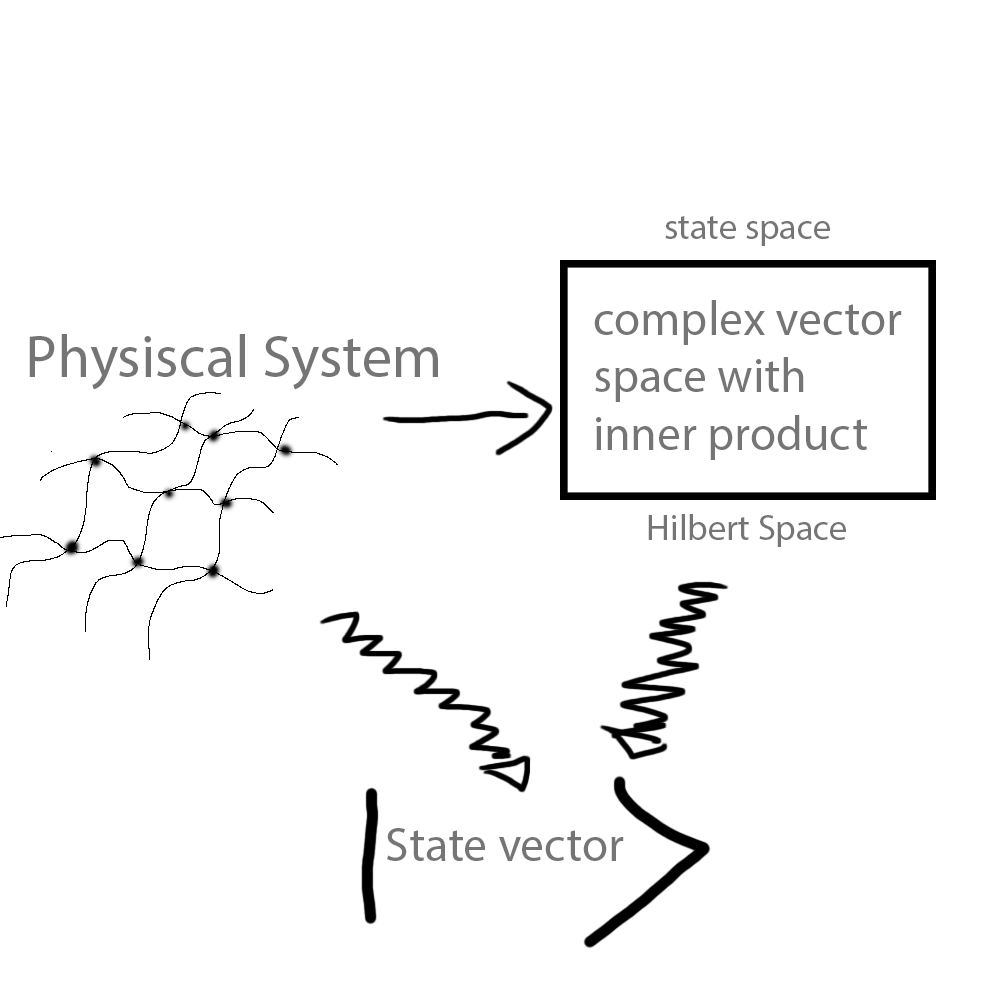
\includegraphics[scale=0.2]{images/sketch1.png} 
%		\caption{how a physical state is represented}
%	\end{figure}
	Every pure quantum state can be represented a vector in a vector space with inner product, i.e. a \emph{Hilbert space}. 
	The implication of this will be explained in the next section; for now we only look of this vector representation.\\
	 A complex Hilbert space $\H$ of dimension $n$ is isomorphic to $ \mathbb{C}^n $ with the standard inner product. 
	 In $\mathbb{C}^n $ one can choose a basis and then represent vectors with coordinates with respect to this basis.\\
	The bra-ket notation is a handy notation introduced by physicist Paul Dirac to deal with such vector representation of quantum states. 
	First of all we note that a state $\varphi '\in\H$ corresponds via the isomorphism to $ \varphi  \in \mathbb{C}^n $. It can be represented as a vector with respect of some basis as follows
	$$\ket{\varphi} = \begin{pmatrix} \varphi_1 \\ \varphi_2 \\ \vdots \end{pmatrix}	  \text{  is a coloumn "ket" vector over } \H $$
	$$\bra{\varphi}  = \begin{pmatrix} \varphi_1 & \varphi_2 & \hdots \end{pmatrix} \text{  is a row "bra" vector over } \H $$
	To be representative of a quantum state the vector has to have unitary length, $\|\varphi\|= 1$.
	Furthermore the conjugate transpose of a \emph{bra} vector is the corresponding \emph{ket} vector, and vice versa.
	$$ \bra{\varphi}^{\dagger} = \ket{\varphi} \text{,    } \ket{\varphi}^{\dagger} = \bra{\varphi}$$
	More specifically, for a complex vector space as $\H$, the components of $\bra{\varphi}$ are each the complex conjugate of the components of $\ket{\varphi}$.\\
	It is worth noting that in quantum information we will consider only vectors of finite dimensions, and more often than not, the standard basis for qubits represented by
	$$\ket0 =  \begin{pmatrix} 1 \\ 0 \end{pmatrix}
	\text{ and }
	\ket1 =  \begin{pmatrix} 0 \\ 1 \end{pmatrix}$$
	which are recognizable as the equivalent of $\vec{e_1}$ and $\vec{e_2}$ in $\mathbb{C}^2$.\\
	
	To summarize then, $\ket{\varphi}$ represents a column vector on a complex vector space with inner product equivalent to $\mathbb{C}^n$ in some basis, and $\bra{\varphi}$ is its complex conjugate.
	
	
	\subsubsection*{Inner/outer product}
	%This one first to start from standard notation
	In standard vector notation we define the inner (scalar) product of complex vectors as
	$$ ( \vec{v}, \vec{w} ) =  \begin{pmatrix} \bar{v_1} & \bar{v_2}\end{pmatrix} \begin{pmatrix} w_1 \\ w_2 \end{pmatrix} = \begin{pmatrix} \bar{w_1} & \bar{w_2}\end{pmatrix} \begin{pmatrix} v_1 \\ v_2 \end{pmatrix} = ( \vec{w}, \vec{v} )^{\dagger}$$
	Written in bra-ket notation, the inner product of two state vectors $\ket{v}$ and $\ket{w}$ is
	$$ ( \ket{v} , \ket{w} ) = \bk{v}{w} = (\ket{w} , \ket{v} )^{\dagger} = \bk{w}{v}^{\dagger} $$
	Where $\dagger$ represents the conjugate transpose,	which produces a scalar (complex) value.\\ %real??
%	This property is fundamental in the sense that it will allows us to go from a state space --- that can be many dimensional --- to a \textit{measurement} space, which assumes real values.\\ %0 and 1 in our case??
	
	It is important also to note that through the inner product of two vectors we also define the norm $\|\ket{v}\|  =  \sqrt{\braket{v}{v}} $.\\
	
	
	The outer product of two vectors, on the other hand, produces a matrix, with very important properties. So if we define the matrix\footnote{The fact that the result of  $ \ketbra{w}{v} $ is indeed a matrix can be seen more directly if we remember that this is nothing less than a column-row vectors multiplication.} $A =  \ketbra{w}{v} $ we observe that
	$$ \ket{w}\braket{v}{v'} = \braket{v}{v'}\ket{w} $$	
	which is a convenient way of visualizing the action of matrix $A$. In particular if we divide it like $(\ketbra{w}{v}) (\ket{v'}) $ it is easy to interpret it as \textit{matrix $A$ acting on vector $\ket{v'}$}; but the other equivalent form $(\braket{v}{v'})(\ket{w})$ can also be seen as multiplying vector $\ket{w}$ by a value $\braket{v}{v'}$. \\
	%this part may be too similar to book, page 67...
	The meaning of this is that $\ketbra{w}{v}$ can indeed be defined as a (linear) operator from the vector space of $\ket{v}$ and $\ket{v'}$ to the vector space of $\ket{w}$. This comes in very handy when we later use it to define operations and measurements on quantum states.\\ % is this true?
	
	\subsubsection*{Linear operators}
	A linear operator between two vector spaces is defined as 
	$$ \mathbf{A}: V\longrightarrow W \text{  ,  }\ket{v_i}\mapsto A\ket{v_i}$$
	$$ \text{ linear in all inputs, i.e.  }  A\left( \sum_i a_i\ket{v_i}\right) = \sum_i a_i A\ket{v_i} \text{  for all } i $$ 
	Looking back at the definition of the matrix $ A = \ketbra{w}{v}$ we can now refer to it as a linear operator from now on. \\
	Some well-known linear operators acting on single qubits that we will use later on are the \textit{Pauli Matrices}
	$$ I = \begin{bmatrix} 1 & 0 \\ 0 & 1 \end{bmatrix}	 \quad   X = \begin{bmatrix} 0 & 1 \\ 1 & 0 \end{bmatrix}$$
	$$ Y= \begin{bmatrix} 0 & -i \\ i & 0 \end{bmatrix}	 \quad   Z = \begin{bmatrix} 1 & 0 \\ 0 & -1 \end{bmatrix}$$
	
	In particular it is safe to say that, unless stated otherwise, the operators that will be presented all have a set of properties and are called Hermitian operators, or self-adjoint operators.\\
	$$ A = A^{\dagger} \quad \Longrightarrow (A\ket{v})^{\dagger} = \bra{v}A^{\dagger} $$ 
	Operators have also to be positive, this means that it holds, for every $\ket{v}$ : $\bra{v}A\ket{v}$ is real non-negative. Any positive operator is also self-adjoint and therefore it has diagonal (spectral) representation $\sum_i \lambda_i \proj{i}$ with non-negative eigenvalues $\lambda_i$.\\
	
	\subsubsection*{Tensor product}
	The tensor product $V\otimes W$ is an operation between vector spaces that combines every element of the first vector space and every element of the second vector space in a bigger vector space. Tensor product is linear and from its properties emerges the famous phenomenon of quantum entanglement, which simply is that not all vectors in $\H = V\otimes W$ can be divided into $\ket{v}\otimes\ket{w}$ with $\ket{v}\in V,\; \ket{w}\in W$. This will later be explained in the next section.\\
	Notation and abbreviation for the tensor product is 
	$$ \ket{v}\otimes\ket{w} = \ket{v}\ket{w} = \ket{v,w} = \ket{vw}$$
	It has the following properties:
	\begin{description}
		\item $\forall\ket{v}\in V ,\; \forall\ket{w}\in W, \; \forall z\in \mathbb{C}$	\\
					$ z(\ket{v}\otimes\ket{w}) = (z\ket{v})\otimes\ket{w} = \ket{v}\otimes(z\ket{w} $
		\item $\forall\ket{v_1},\ket{v_2}\in V ,\; \forall\ket{w}\in W$	\\
					$ (\ket{v_1} + \ket{v_2})\otimes\ket{w} = \ket{v_1w} + \ket{v_2w} $
		\item $\forall\ket{v}\in V ,\; \forall\ket{w}\in W, \; A:V\rightarrow V' \; B:W\rightarrow W'$	\\
					$ (A\otimes B) \left(\sum_i a_i \ket{v_i w_i} \right) = \sum_i a_i A\ket{v_i}\otimes B\ket{w_i} $
	\end{description}
	The inner product on $V$ and $W$ can be used to define (linearly) an inner product on $V\otimes W$.	
	
\section{Quantum Mechanics}
	%TODO Correct and reformulate this
	
	\begin{quotation}
		The simplest quantum mechanical system, and the system which we will be most concerned with, is the \emph{qubit}. A qubit has a two-dimensional state space. [...] 
		The way a qubit differs from a bit is that superpositions of these two states, of the form $a\ket{0} + b\ket{1}$, can also exist, in which it is not possible to say that the qubit is definitely in the state $\ket0$, or definitely in the state $\ket1$.
		\cite{NC10}
	\end{quotation}
	
	\subsubsection*{The three postulates}
	\begin{quote}
		\textbf{Postulate 1}: Associated to any isolated physical system is a complex vector space with inner product (that is, a Hilbert space) known as the \emph{state space} of the system. 
		The system is completely described by its \emph{state vector}, which is a unit vector in the system's state space. \cite{NC10}
	\end{quote}
	
	\begin{quote}
		\textbf{Postulate 2}: The evolution of a \emph{closed} quantum system is described by a \emph{unitary transformation}. That is, the state $\ket{\psi}$ of the system at time $t_1$ is related to the state $\ket{\psi'}$ of the system at time $t_2$ by a unitary operator $U$ which depends only on times $t_1$ and $t_2$,
		$$ \ket{\psi'} = U\ket{\psi} $$
		\cite{NC10}
	\end{quote}
	
	\begin{quote}
		\textbf{Postulate 3}: Quantum measurements are described by a collection $\{M_m\}$ of \emph{measurements operators}. 
		These are operators acting on the state space of the system being measured. 
		The index $m$ refers to the measurement outcomes that may occur in the experiment. If the state of the quantum system is $\ket{\psi}$ immediately before the measurement then the probability that result $m$ occur is given by 
		$$ p(m) = \bra{\psi}M_m^{\dagger}M_m\ket{\psi} \: ,$$
		and the state of the system after the measurement is 
		$$ \frac{M_m\ket{\psi}}{\sqrt{\bra{\psi}M_m^{\dagger}M_m\ket{\psi}}} \: . $$
		The measurement operators satisfy the \emph{completeness equation},
		$$\sum_m  M_m^{\dagger}M_m = I \: .$$
		The completeness equation expresses the fact that probabilities sum to one:
		$$ 1 = \sum_m p(m) = \sum_m  \bra{\psi}M_m^{\dagger}M_m\ket{\psi} \: .$$ 
		\cite{NC10}
	\end{quote}
	
	Quantum mechanics is a very large and complex theory. For our purposes it is enough for us to only consider the quantum system called \emph{qubit} and its rules of computation following from the tensor product algebra.  ...
	
	%TODO review this
	All pure states in QM are normalized vectors in $\H$.
	$$ \ket{\psi} \text{ is a state vector } \Rightarrow \ket{\psi}\in\H \text{ and }  \vert\bk{\psi}{\psi}\vert = 1$$
	This is instrumental in seeing them as probability vectors. Every linear operator has then to be unitary to maintain this property.\\
	A statistical mixture of states corresponds to a \emph{density matrix}, which is itself a new state. It is important to note that a mixture of probability of states is not the same thing as superposition of states. In the latter we don't have a measure of uncertainty of the state, meaning also that in theory we are always able to find a measurement basis that will always output the same result for that state. In the former, however, this is not possible given by the direct intrinsic uncertainty of the state.\\
	Density matrices have then the properties:
	$$ M = \rho = \sum_i p_i \ketbra{\psi_i}{\psi_i} = \sum_i p_i P_{\ket{\psi_i}} \text{  , where state }\ket{\psi_i}\text{ has probability } p_i $$ 
	$\rho$ is a positive, trace-1 operator meaning that $\Tr{\rho} = 1$ and all eigenvalues of $\rho$ are positive. Moreover $\rho$ is a linear combination of projectors $\proj{\psi_i}$ which makes $\rho\in\mathbf{P}(\H)$ a projector itself on the the Hilbert space.
	
		\subsection{Quantum Measurements}
		To get an actual value out of a qubit one has to \textit{measure} it. Measurement is, mathematically, a projection onto some chosen computational basis. The result for each base vector projection is then interpreted as a \emph{probability}. The state then changes after measurement, meaning for example that it will not retain it value as superposition any more.\\
		...\\
		
		If Alice has the state $\ket{psi_i}$ out of $i=1..n$ and all states are orthonormal, then Bob can find out what the choice of $i$ was.
		If the states are not orthonormal there is no quantum measurement capable of distinguishing the states. \\
		From this follows that if the states $\ket{\psi_1}$ and $\ket{\psi_2}$ are not orthogonal, then $\ket{\psi_2}$ has a component orthogonal to $\ket{\psi_1}$ but also a component parallel to it which will give probability not $0$ of measuring differently.
		
			\begin{xmpl}
      \begin{equation*} % environment for equation 
				Z = \begin{bmatrix} 1 & 0 \\ 0 & -1 \end{bmatrix} \quad P_{+1} = \proj{0} , \; P_{-1} = \proj{1}
      \end{equation*}
				Measurement on qubit $ \ket{\psi} = \frac{\ket0 + \ket1}{\sqrt{2}} $ has probability $p_{+1} = \bra{\psi}P_{+1}\ket{\psi} = \bk{\psi}{0}\bk{0}{\psi} = \frac{1}{2}$ and similarly $p_{-1} = \frac{1}{2}$
				\cite{NC10}
			\end{xmpl}

		\subsection{Quantum Entanglement}
		\begin{quotation}
		There exist vectors in $V\otimes W$ that can not be represented by a single tensor product:
		Given $v_1,v_2\in V \; w_1,w_2\in W$ linear independent:
    \begin{equation*}
		v_1\otimes w_1 + v_2\otimes w_2 = v_1w_1 + v_2w_2 \in V\otimes W
    \end{equation*}
    is \emph{not} separable.
		this may be strange because on physical level tensor product is combination(merging) of quantum systems (??? this is not a complete sentence??)
		\end{quotation}
		\cite{Han13}
		
		\begin{figure}[h]
			\centering
			%% Little schematics showing the origin of entanglement
%% from the linear theory of QM and tensor product

\begin{tikzpicture}[scale=0.6]
  \node[colorbox=red]                      (lin)  {Linearity};
  \node[colorbox=magenta, below=.5cm of lin] (tp)  {Tensor product};
  \node[colorbox=blue, below=.5cm of tp]   (en)  {Entanglement};
  \draw[conn=2pt, densely dotted] (tp) to (lin);
  \draw[conn=2pt, densely dotted] (en) to (tp);
\end{tikzpicture}
			\caption{origin of entanglement via linearity}
		\end{figure}
	
\section{Information Theory}
	
	\subsection{Mutual Information}
	Mutual information can be used as a measure of correlation between random variables. 
	
	Mutual information is defined as
	$$ I(X;Y) = \sum_{y\in\mathcal{Y}}\sum_{x\in\mathcal{X}} p(x,y) \log\left(\frac{p(x,y)}{p(x)p(y)}\right) $$
	or equivalently, showing its relation to the entropies of the random variables
	$$ I(X;Y) = H(X) - H(X\mid Y) = H(X,Y) - H(X\mid Y) - H(Y\mid X) $$
	This relation can be seen more directly in Fig. \ref{fig:mutual_info}.\\
	Mutual information is nonnegative and bounded by the entropy of random variable $X$
	$$ 0 \leq I(X;Y) \leq H(X) $$
	In this sense mutual information can also be interpreted as how much measuring one variable reduces the uncertainty of the other, thus being bounded by its uncertainty itself.
	
	\begin{figure}[h]
		\centering
		% Representation of mutual information in relation to entropy of variables
\tikzset{colorcircle/.style={circle, thick, minimum size=4cm, text height=1.7ex,text depth=.25ex, text width=3cm, draw=#1!70!black, fill=#1!30, fill opacity=0.33, text opacity=1.0}}

\begin{tikzpicture}[scale=0.6]
  
  \node[colorcircle=magenta] (Hx) at (-2,0)  {$ H(X\mid Y) $ \hfill};
  \node[colorcircle=blue] (Hy) at (2,0)  {\hfill $ H(Y\mid X) $};
  \node (mI) at (0,0) {$ \mathbf{I(X;Y)} $};
  \node [left =of Hx.north] (HxL) {$ H(X) $};
  \node [right =of Hy.north] (HyL) {$ H(Y) $};
  \node (Hxy) at (0,-5.5) {$ H(X,Y) $};
  \draw[->] (Hxy.north) -- ( Hx.south);
  \draw[->] (Hxy.north) -- (Hy.south);
\end{tikzpicture}
		\caption{Representation of mutual information $I(X;Y)$ in relation with entropies $H(X)$ and $H(Y)$ and joint entropy $H(X,Y)$ of the random variables .
		\label{fig:mutual_info}}
	\end{figure}		
	
	\subsection{Common Secret} \label{commonsecret}%here?
	Let $X,Y,Z,S$ be random variables on the same range $\mathcal{X}$. Let $X$ be owned by Alice, $Y$ by Bob and $Z$ by Eve. Then
  \begin{align}
	 & P[X=Y=S] > 1 - \epsilon\label{eqn:common}\tag{common} \\ 
	 & I(X;Z) = 0 \: \wedge \: I(Y;Z) = 0 \label{eqn:secret}\tag{secret}
  \end{align}
for all $\epsilon > 0 $. \\
The first part defines the \textit{common} property: $X$ and $Y$ must be asymptotically the same. 
The second part states that the amount of information Eve can gather about $X$ and $Y$, through it's realization of $Z$, is $0$.
